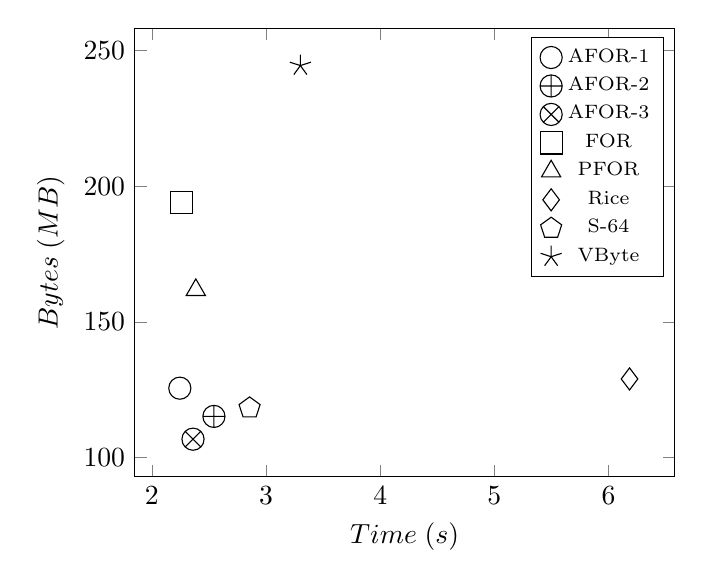
\begin{tikzpicture}
\begin{axis}[
	scatter/classes={
	a={mark=o},
	b={mark=oplus},
	c={mark=otimes},
	d={mark=square},
	e={mark=triangle},
	f={mark=diamond},
	g={mark=pentagon},
	h={mark=star}
  },
  ylabel=$Bytes \; (MB)$,
  xlabel=$Time \; (s)$,
  mark options={scale=2},
  legend style={font=\scriptsize},
]

\addplot[only marks]
plot[scatter, scatter src=explicit symbolic]
coordinates {
 (2.2446, 125.6) [a]
 (2.5433, 115.2) [b]
 (2.36, 106.8) [c]
 (2.257, 194.0) [d]
 (2.3846, 161.8) [e]
 (6.1836, 129.0) [f]
 (2.8555, 118.3) [g]
 (3.3004, 244.5) [h]
};
\legend{AFOR-1, AFOR-2, AFOR-3, FOR, PFOR, Rice, S-64, VByte}
\end{axis}
\end{tikzpicture}